\begin{figure}
    \begin{center}
    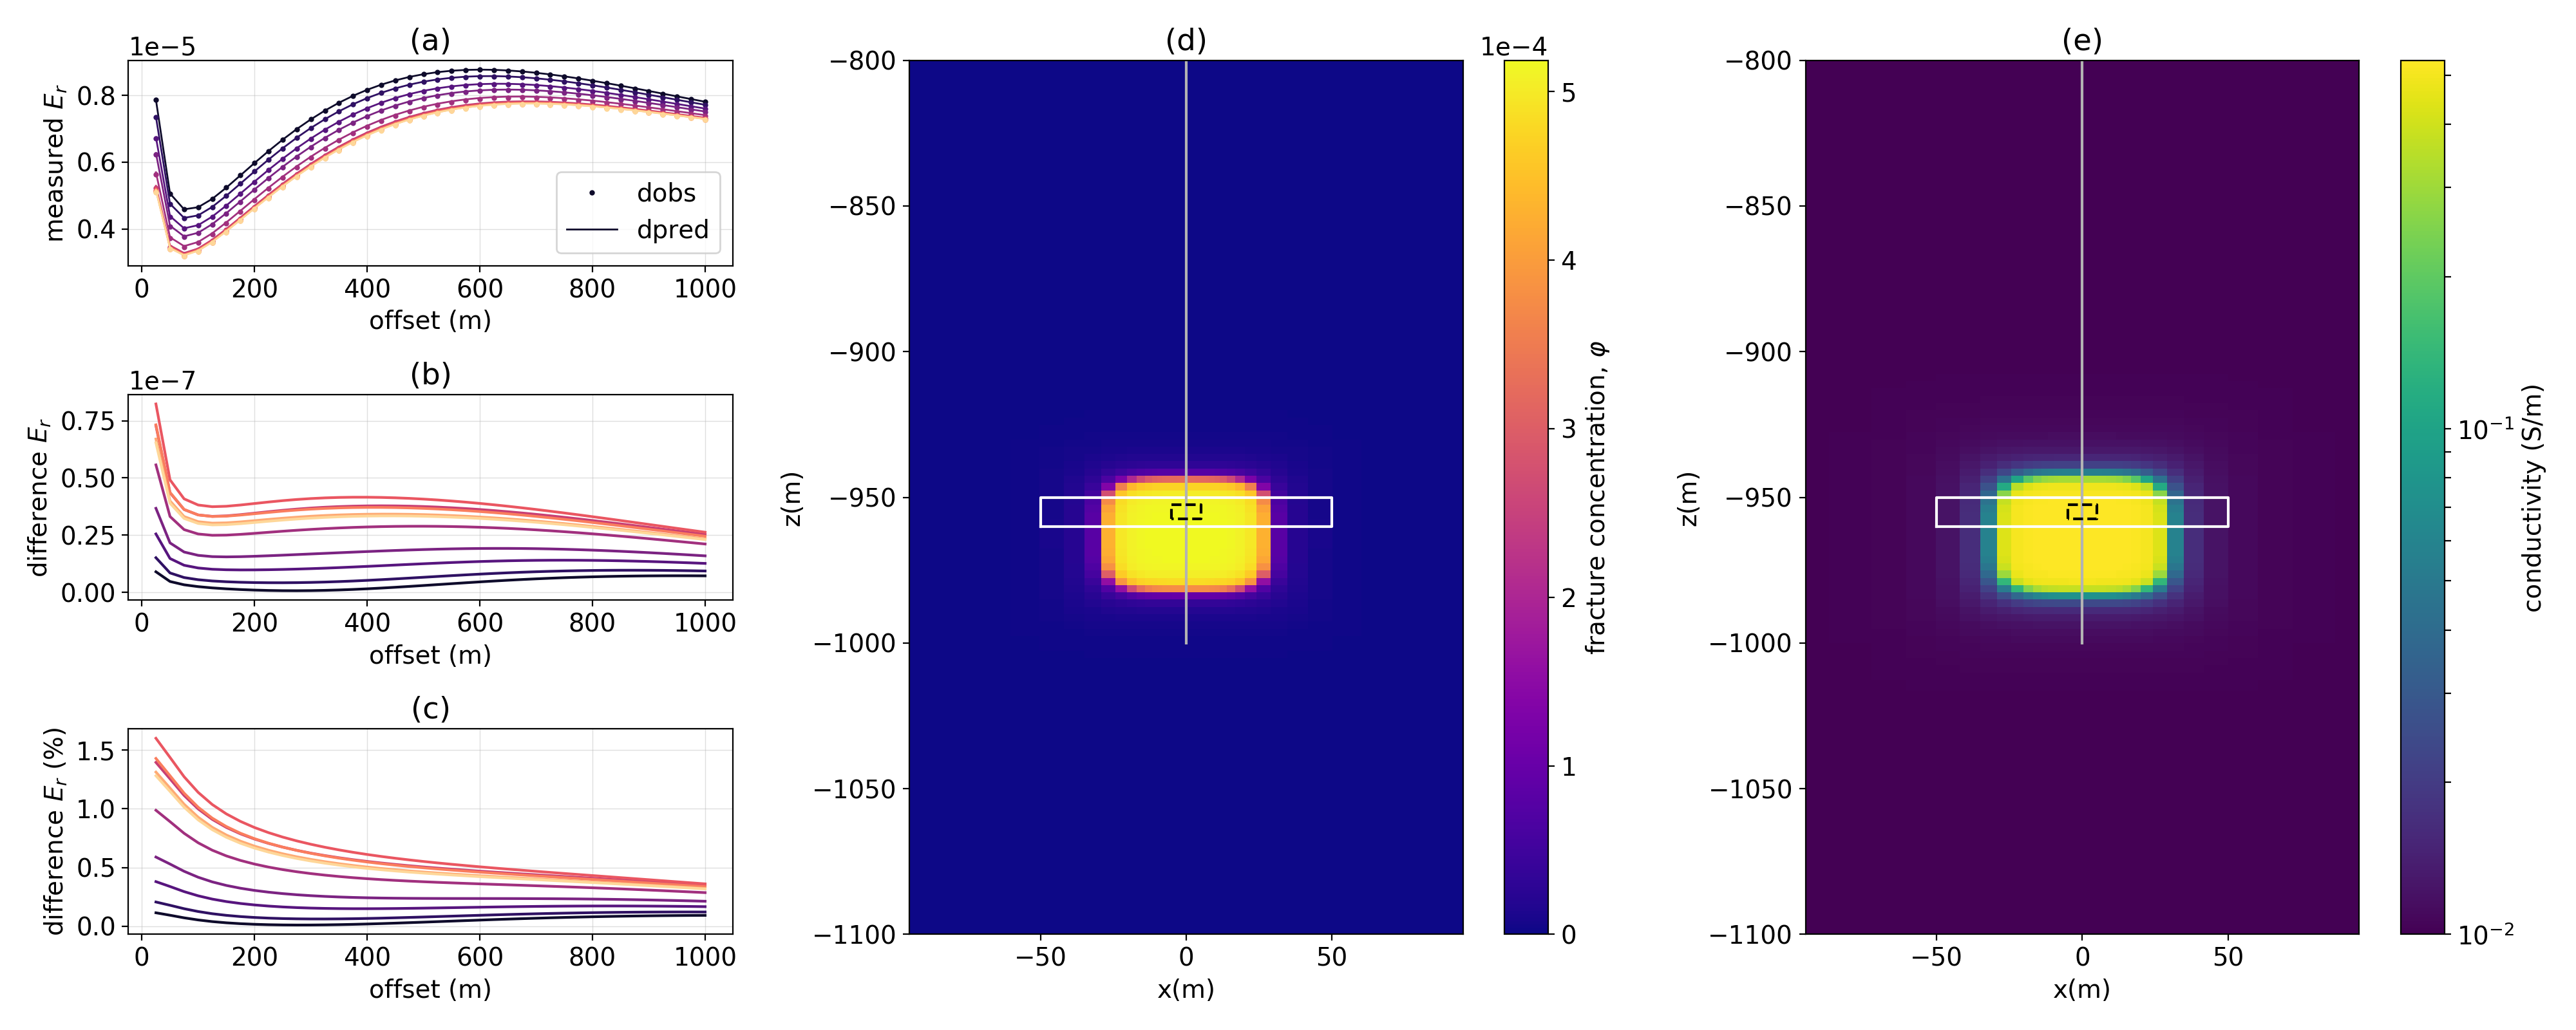
\includegraphics[width=\textwidth]{figures/inversion/dc_parametric_inversion_phi_correctz0.png}
    \end{center}
\caption{
    Inversion result using a parametric model of the fracture concentration. The concentration is
    converted to electrical conductivity using the effective medium theory mapping shown in
    equation \ref{eq:effective_medium_theory_mapping}.
    The black dashed line outlines the geometry of the starting model. The initial fracture concentration
    is $10^{-10}$ in the background and $10^{-4}$ in the target.
    The data are fit to a global $\chi$-factor $<$ 0.05 and the inversion took 12 iterations.
}
\label{fig:dc_parametric_inversion_phi_correctz0}
\end{figure}
